\chapter{Modelling of {\prox} spectra}
\protect\label{chapter:modelling}
\lhead{Chapter \ref{chapter:modelling} \emph{Modelling of {\prox} spectra}}

In order to develop and refine the methods for evaluation of the periodicity of the sub-peaks in the {\prox} spectra, a
version of the ``Doppler Tomography of Stars'' (DoTS) modelling software \citep{CCamerondotsa} was used. Although DoTS
was written to recover surface imhomogeneities from time series spectra, here the forward modelling routines were used
to generate synthetic spectra, with some modifications. Specifically, \examrevision{a 3D model of the star, but with a 2D
  spherical model of the photosphere} was constructed, covered in a finite number of pixels. The intensity of each pixel
can vary from a photospheric value to a value appropriate for plage. In order to obtain the appropriate photospheric
intensity for each pixel at a given rotation phase of the stellar model,the 4-parameter limb darkening law introduced by
Claret from Phoenix model atmospheres \citep{claret00a} was used for an effective temperature of 3000K. The plage
intensities were calculated according to \citet[Section 4.1]{unruh99}, who identified the centre to limb variability
from plage regions relative to the photospheric (quiet) intensity for the Sun. Since no such observations exist for
other stars, the same \examrevision{centre-to-limb variation as for the solar plage was used relative to the photospheric
  centre-to-limb variation of \prox, selecting the limb-darkening law appropriate for the lower photosphere temperature
  and} with appropriate facular contrasts for {\ha} wavelengths (see \citet[figs 3 \& 4]{unruh99}).

Since it was desired to simulate the {\ha} line profile, a local intensity profile was assumed for the photosphere and
the plage. For inactive photospheres of \rdwarf s with similar spectral type to {\prox}, {\ha} is not visible (e.g. see
{\ha} profile in \citet[fig. 6]{barnes14} for GJ1061). Hence for the quiet photosphere, a flat continuum was assumed For
active stars, {\ha} possesses a characteristic emission profile with self-absorption, resulting in a double-peaked
profile. Since the {\vsini} is probably less than 0.1 km/s for \prox, the local line profile shape for {\ha} was based
on the observed {\prox} line profile since it is unlikely to show rotational broadening. This profile was tuned to
resemble the average {\ha} profile shown in the {\uves} data analysed in \citet{fuhrmeister11}, but symmetric about the
central wavelength. Specifically, a Gaussian profile was used to generate the emission peak and a second Gaussian with
narrow width to represent the central self-absorption as illustrated in Fig. \ref{fig:integregions}.  \examrevision{The
  profile was selected with the spread of wavelengths in resembling the {\ha} peak and with equivalent width so as to
  resemble the mean peak in the {\harps} data. The intensity could be fine-adjusted in the lookup-table parameters for
  the DoTS program so as to yield a variation in equivalent width comparable to that of the {\harps} observations
  ignoring those affected by flares with the selected plage distribution in use.}

\begin{figure}[!htbp]
\begin{center}
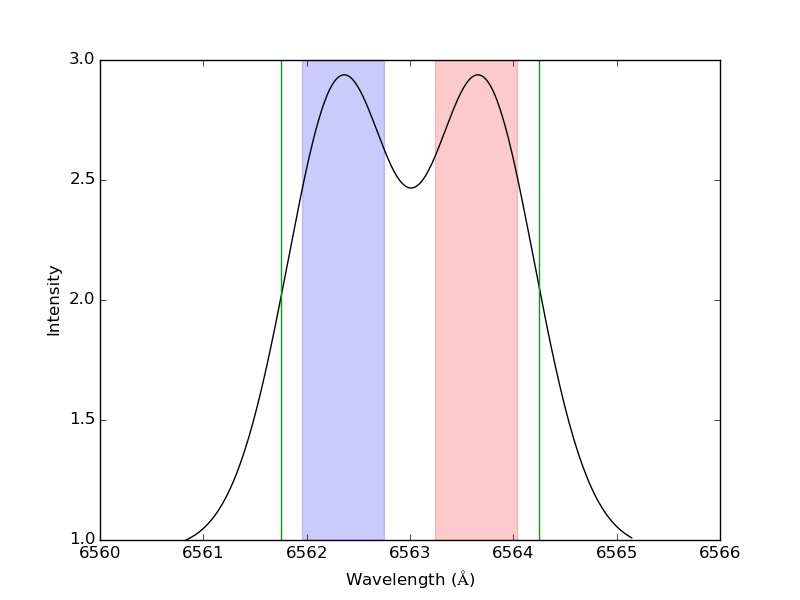
\includegraphics[scale=0.40]{Figures/integregions.png} \\
\end{center}
\caption{Example generated model spectrum of \prox, also illustrating the methods for computing the periodicity of
  spectra.  The centre of the \ha{} line is set at 6563{\AA} for convenience rather than 6562.8\AA{}.  The green lines
  (from 6561.75{\AA} to 6564.25\AA) show the limits used for calculation of the equivalent width. The blue and red
  shaded areas (6561.95{\AA} to 6562.75{\AA} and 6563.44{\AA} to 6564.24{\AA} respectively, each 0.8{\AA} wide) show the
  regions for calculation of the peak ratio.}
\protect\label{fig:integregions}
\end{figure}
% Done with 10 plage 80 period 75 deg first spectrum

With the two-temperature model, in subsequent simulations below, either photospheric intensity or a plage intensity is
assigned to each pixel. For a pixel containing plage, the synthetic {\ha} profile is scaled and for the photosphere with
no visible profile (as note above), the continuum level is used. The line profile is shifted appropriately for the
Doppler shift of each pixel in the model, \examrevision{however with the small Doppler shift due to the {\vsini} of less
  than 0.1 km/s on {\prox}, the main velocity variation observed is due to the asymmetry of the plage distribution}. The
model enables the user to place circular spots of specified radii anywhere on the star. For each viewing angle (or
equivalently observation phase), the appropriate intensity profiles of all visible pixels is calculated (according to
position on the line and centre-to-limb variation) and sum them to obtain the simulated line profile.

A model star with plage regions that rotate into and out of view can thus potentially exhibit variability in the line
shape since the pixels on different parts of the star possess different Doppler velocities. For stars such as \prox,
which probably possess a {\vsini} much less than the instrumental resolution, \examrevision{any velocity distortions in
  the the line profile due to spots rotating into and out of view will be insignificant or very small}. A plage region
that rotates into view may nevertheless have a significant effect on the the equivalent width of the simulated line
since the local intensity profile for {\ha} \examrevision{possesses a greater normalised peak intensity than} the
continuum. For stars with rotational velocity much greater than the instrument resolution, line asymmetries are likely
to be much more reliable.

\section{Plage distribution and results}
\protect\label{section:plagedists}

During the course of experimentation with models, a selection of plage distributions was tried, ranging from a single
large spot on one face to randomly-placed spots of random sizes. \examrevision{In all cases a 100\% filling factor for
  the plage was selected.} However it was found that the variation in equivalent widths from a low spot coverage was
bore no possible resemblance to that from observational data, in that the generated simulated spectra just exhibited two
extremes of equivalent widths and no intermediate values. On the other hand a coverage of more than about 30\% provided
very limited swings in the equivalent width compared those observed from {\harps} and {\uves}. After some
experimentation, a randomly distributed plage was settled upon which \examrevision{covered} up to 2.5\% of the surface,
towards the high end of the coverage of up to 2.7\% reported in \citet{guttenbrunner14} in relation to the Sun,
\examrevision{with the intensity parameters in the flux profile and the model adjusted to yield a variation in equivalent
  widths similar to the {\harps} observations}.

The models were all generated with the observation dates from the Original Set of {\harps}\footnote{This work was
  completed before the 2016 data was available. Also, as discussed in Section \ref{section:addflares}, it proved useful
  to study the Original Set of data as the 116.6 day period of \citet[Table 3]{suarezmascareno15} appeared in some
  cases, as illustrated in Fig. \ref{fig:rec116}.}, using possible rotation periods between 15 and 90 days in steps of 5
days and inclinations between 10{\degree} and 90{\degree} in steps of 5{\degree} to observe the various effects. Only a
limited selection, usually multiples of 10 days and 10{\degree} are shown in this {\paperorthesis} to conserve space.

In Fig. \ref{fig:extremew} some example spectra showing extremes of equivalent width and the median  are shown, and in
Fig. \ref{fig:extremewpics} the corresponding visible faces of the star with the plage spots marked in.

\begin{figure}[!htbp]
\begin{center}
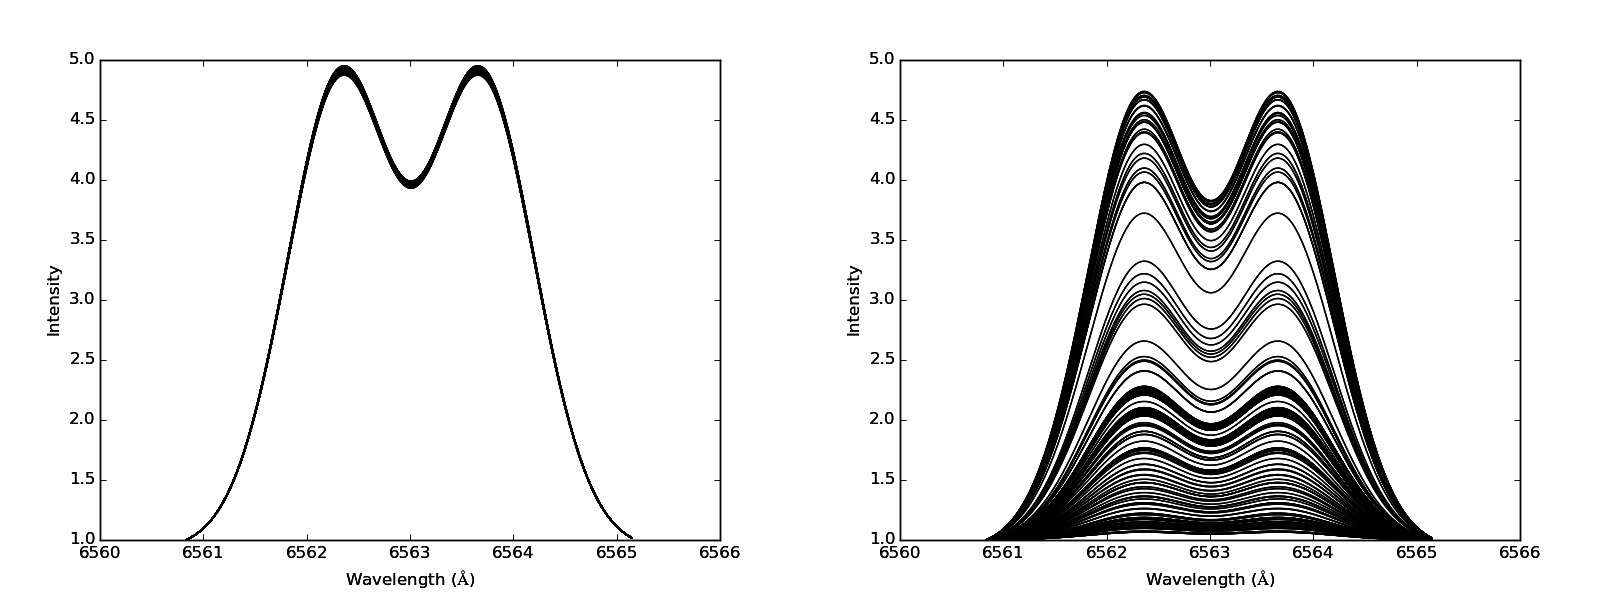
\includegraphics[scale=0.40]{Figures/extremes.png} \\
\end{center}
\caption{This displays simulated spectra showing the extremes and the median value of equivalent width (1.5, 3.0 and 2.3
  respectively) with a period of 80 days and an inclination of 80\degree. The epochs from the {\harps} data are used in
  the model and the selected generated spectra superimposed.}
\protect\label{fig:extremew}
\end{figure}

\begin{figure}[!htbp]
\begin{center}
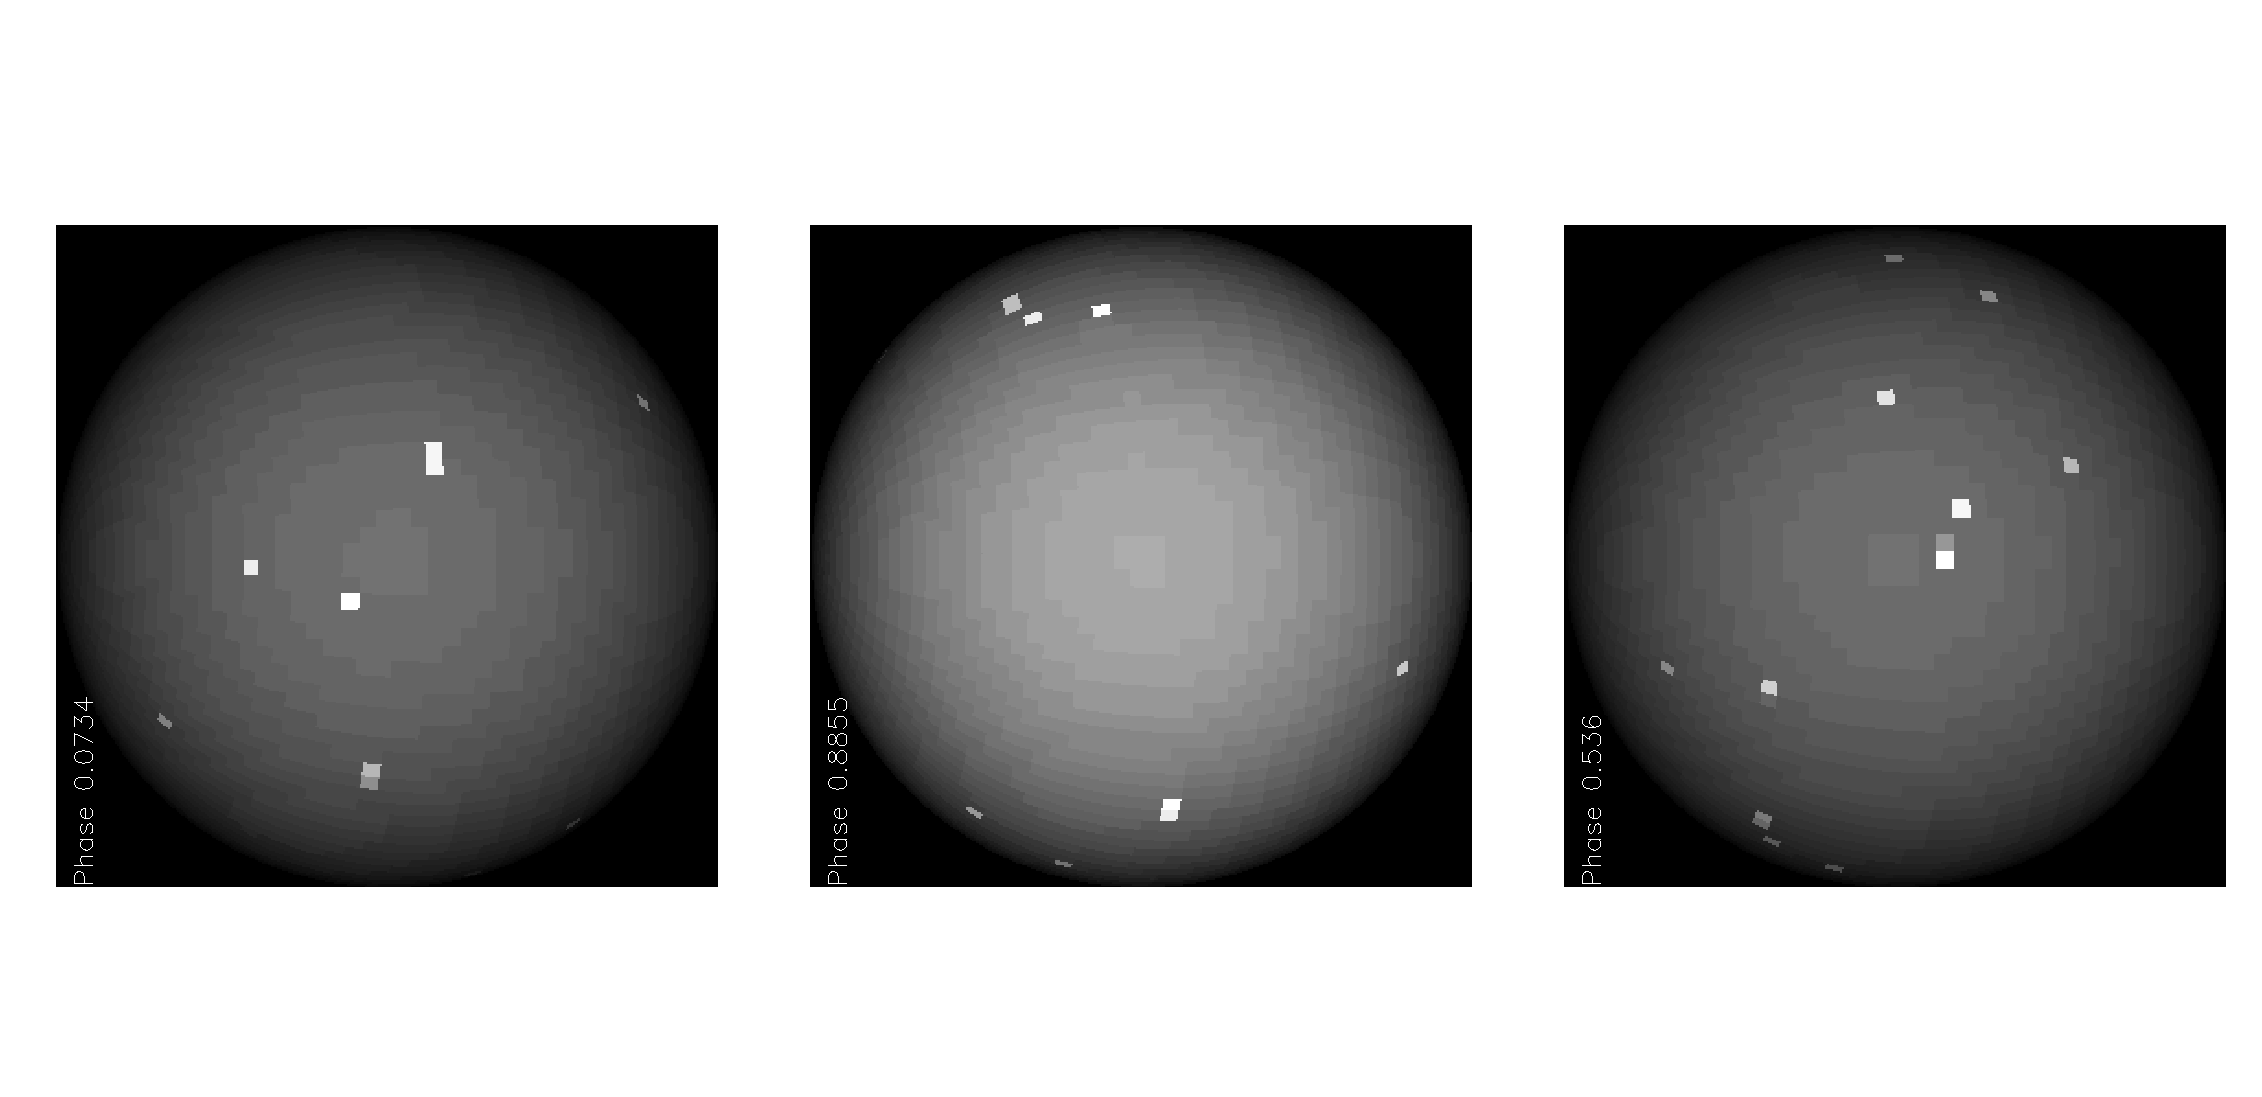
\includegraphics[scale=0.18]{Figures/extremeewpics.png} \\
\end{center}
\caption{This shows the visible face of the star as generated by DoTS corresponding to the spectra displayed in
  Fig. \ref{fig:extremew} in chronological order. Left to right, these give the spectra with the median, the lowest and
  the greatest equivalent widths.}
\protect\label{fig:extremewpics}
\end{figure}

In table \ref{table:modelcomp} are presented a selection of typical results showing means and standard deviations
for the equivalent width method (EW) with the two plage distributions for various periods and with 30{\degree},
60{\degree} and 90{\degree} inclinations and for 70, 80 and 90-day periods with 10{\degree} to 90{\degree} inclinations.
Note that the PR results are not displayed as variations were insufficient to be displayed in less than 6 figures, the
Doppler variations are just too insubstantial.

\begin{table}[!htbp]
\centering
\scalebox{0.75}{
\begin{tabular}{|l|c|l|l|l|}
\hline
Plage Dist & Period & \multicolumn{1}{|c|}{30\degree}&\multicolumn{1}{|c|}{60\degree}&\multicolumn{1}{|c|}{90\degree}\\\hline
\multirow{8}{*}{Random to 2.5\%} & 20 & 2.150 $ \pm $ 0.572 & 2.746 $ \pm $ 0.939 & 2.735 $ \pm $ 0.891  \\
& 30 &  2.725 $ \pm $ 0.495 & 3.870 $ \pm $ 0.895 &  4.004 $ \pm $ 0.942 \\
& 40 &  1.917 $ \pm $ 0.541 & 2.501 $ \pm $ 0.927 &  2.614 $ \pm $ 0.967 \\
& 50 &  1.604 $ \pm $ 0.483 & 1.996 $ \pm $ 0.805 &  2.018 $ \pm $ 0.876 \\
& 60 &  1.626 $ \pm $ 0.573 & 2.057 $ \pm $ 0.951 &  2.099 $ \pm $ 1.006 \\
& 70 &  1.967 $ \pm $ 0.445 & 2.334 $ \pm $ 0.803 &  2.340 $ \pm $ 0.821 \\
& 80 &  1.637 $ \pm $ 0.495 & 2.161 $ \pm $ 0.805 &  2.309 $ \pm $ 0.828 \\
& 90 &  2.475 $ \pm $ 0.548 & 3.365 $ \pm $ 0.894 &  3.410 $ \pm $ 0.901 \\\hline
\end{tabular}}

\vspace{5 mm}

\scalebox{0.75}{
\begin{tabular}{|l|c|l|l|l|}
\hline
Plage Dist & Incl\degree & \multicolumn{1}{|c|}{70 days}&\multicolumn{1}{|c|}{80 days}&\multicolumn{1}{|c|}{90 days}\\\hline
\multirow{9}{*}{Random to 2.5\%} & 10 & 1.693 $ \pm $ 0.140 & 1.484 $ \pm $ 0.182 & 1.816 $ \pm $ 0.196 \\
& 20 &  1.811 $ \pm $ 0.292 &  1.492 $ \pm $ 0.356 &  2.116 $ \pm $ 0.387 \\
& 30 &  1.967 $ \pm $ 0.445 &  1.637 $ \pm $ 0.495 &  2.475 $ \pm $ 0.548 \\
& 40 &  2.116 $ \pm $ 0.590 &  1.810 $ \pm $ 0.626 &  2.827 $ \pm $ 0.691 \\
& 50 &  2.237 $ \pm $ 0.711 &  1.994 $ \pm $ 0.732 &  3.139 $ \pm $ 0.815 \\
& 60 &  2.334 $ \pm $ 0.803 &  2.161 $ \pm $ 0.805 &  3.365 $ \pm $ 0.894 \\
& 70 &  2.392 $ \pm $ 0.860 &  2.277 $ \pm $ 0.848 &  3.477 $ \pm $ 0.930 \\
& 80 &  2.396 $ \pm $ 0.877 &  2.338 $ \pm $ 0.850 &  3.464 $ \pm $ 0.911 \\
& 90 &  2.340 $ \pm $ 0.821 &  2.309 $ \pm $ 0.828 &  3.410 $ \pm $ 0.901 \\\hline
\end{tabular}}
\caption{Simulated mean equivalent widths with associated standard deviations from simulations for the 2.7\%
  plage distributions and a set of rotation periods and inclinations. In the first table results are illustrated for
  various periods and for 30{\degree}, 60{\degree} and  90{\degree} inclinations. In the second table results are
  illustrated for various inclinations and 70, 80 and 90-day periods as these are close to the
  rotation period of \prox.}
\protect\label{table:modelcomp}
\end{table}

For each set of generated spectra for both plage distributions, rotation period (between 15 and 90 days in steps of 5
and inclination (between 10{\degree} and 90{\degree} in steps of 5\degree), a periodogram was obtained, viewing periods
between 10 days and 130 days in steps of 0.01 days, from the calculated equivalent widths and the RMS error over all
inclinations noted. In nearly all cases the error was rarely more than 0.02 days. It was rather a different matter for
the peak ratios however, in that the variations observed in the peak ratios were typically $2{\times}10^{-5}$ at most or
with the most extreme plage distributions could be stretched to $2{\times}10^{-4}$. These variations are just above the
level at which it is possible to reliably measure the peak ratio from the observed data but far below the observed peak
ratio changes in the data which are two orders of magnitude higher, e.g. combining all the {\harps} data, a result of
0.997 $ \pm $ 0.018 (one $\sigma$) was obtained.

\examrevision{An attempt was made to reproduce the peak ratio variations by considering an asymmetric pair of Gaussians
  either side of the central wavelength for the plage flux profiles, but in order to achieve the observed variations, a
  vertical velocity approaching 100 km/s would be required. This is well in excess of the speed of sound in the
  chromosphere, estimated for the Sun as approximately 8 km/s \citep{uitenbroek04} and would therefore have to be
  discounted as unphysical.}

\section{Adding in noise and flares}
\protect\label{section:addflares}

Despite the limitations of the simplistic model, \examrevision{some confidence could be expressed in the measurement of
  periodicity from the equivalent width method}, although the peak ratio variations could not be reproduced from a
straightforward model and that method reliably applied.  These results are for a noiseless set of models and to compare
with reality the performance of the modelling results and the analysis methods in the presence of observational noise
and also the influence of simulated flare events has to be considered.

As a first step in moving to something like actual observational data, noise of a given signal to noise ratio was added
to the simulated spectra and the effect observed on the accuracy of the periodicity measurements for various levels,
inclinations and starting periods. Adding Gaussian noise with SNRs from 100 down to 1 in steps of 0.1 was tried.
These were tried with all the combinations of inclinations and starting periods tried before and attempts made to see
how that affected the rate of recovery.

It was noticeable that doing this only started to have any significant effect with SNR below 20. Below this level, two
things started to happen, increasingly as the SNR was reduced. Either the error in the recovered period increased,
although not by very much (typically less than 2\%), alternatively the recovered period was manifestly incorrect, giving
a clear False Positive such as returning a period of 50 days from a starting period of 80 days.

It was easy to discriminate between these two cases by setting a threshold of 5\% for the difference between the
recovered period and the starting period. If the difference exceeded this, then the period was regarded as incorrectly
recovered, otherwise it was regarded as correctly recovered but with the given error. However in all the cases the
difference was either substantially greater or substantially less than this.

Also examined was the possible effect of flares. The effect of flares was simulated by taking the spectra
which were clipped as having excessive equivalent width in Section \ref{section:harpsper}\footnote{N.B. This was done
  with the Original Set of data and observation times as previously noted.} and adding in the same
proportionate excess over the median equivalent width in the model as was found in the observed data. The result was a
poorer performance than with noise alone, but not by much. With just noise, the performance became markedly low with a
SNR of 15 or below but adding flares as described significantly reduced the performance with a SNR of 20 or below. These
values of SNR are much lower than the published values for {\uves} and {\harps}, which are in both cases well over
200\footnote{The calculations of equivalent width, {\ha} Index and peak ratios for {\harps} also calculated the
  uncertainty in the these values, which remained of the same order.}.

In Fig. \ref{fig:noiseresults} is shown the effect of varying SNR and adding in simulated flare data on the rate of
recovery, expressed as a percentage of the correct period of 80 days. Each data point was calculated 100 times with
different randomly-generated noise\footnote{For an exhaustive analysis this would clearly have to be repeated many more
  times, but 100 times seemed adequate for an overview.}. The blue plot shows the effect of just adding
noise, the green that of adding in the four largest flares and noise and the red shows the effect of adding simulated
flares from all the values in the {\harps} data clipped having equivalent width over 3.8. This is illustrated for
inclinations of 30{\degree}, 60{\degree} and 90{\degree}. it can be seen that the smaller inclinations have a
significantly deleterious effect on the rate of recovery especially in the presence of flares.

It should be stressed that this is the rate of recovery of the correct period as the \underline{strongest} peak in the
periodograms, not as one of the top 5 as in, for example, Fig. \ref{fig:photcomp1}. All of the models apart from a
few from the very poorest SNRs of less than 5 at low inclination gave the correct period as one of the top five peaks.

\begin{figure}[!htbp]
\begin{center}
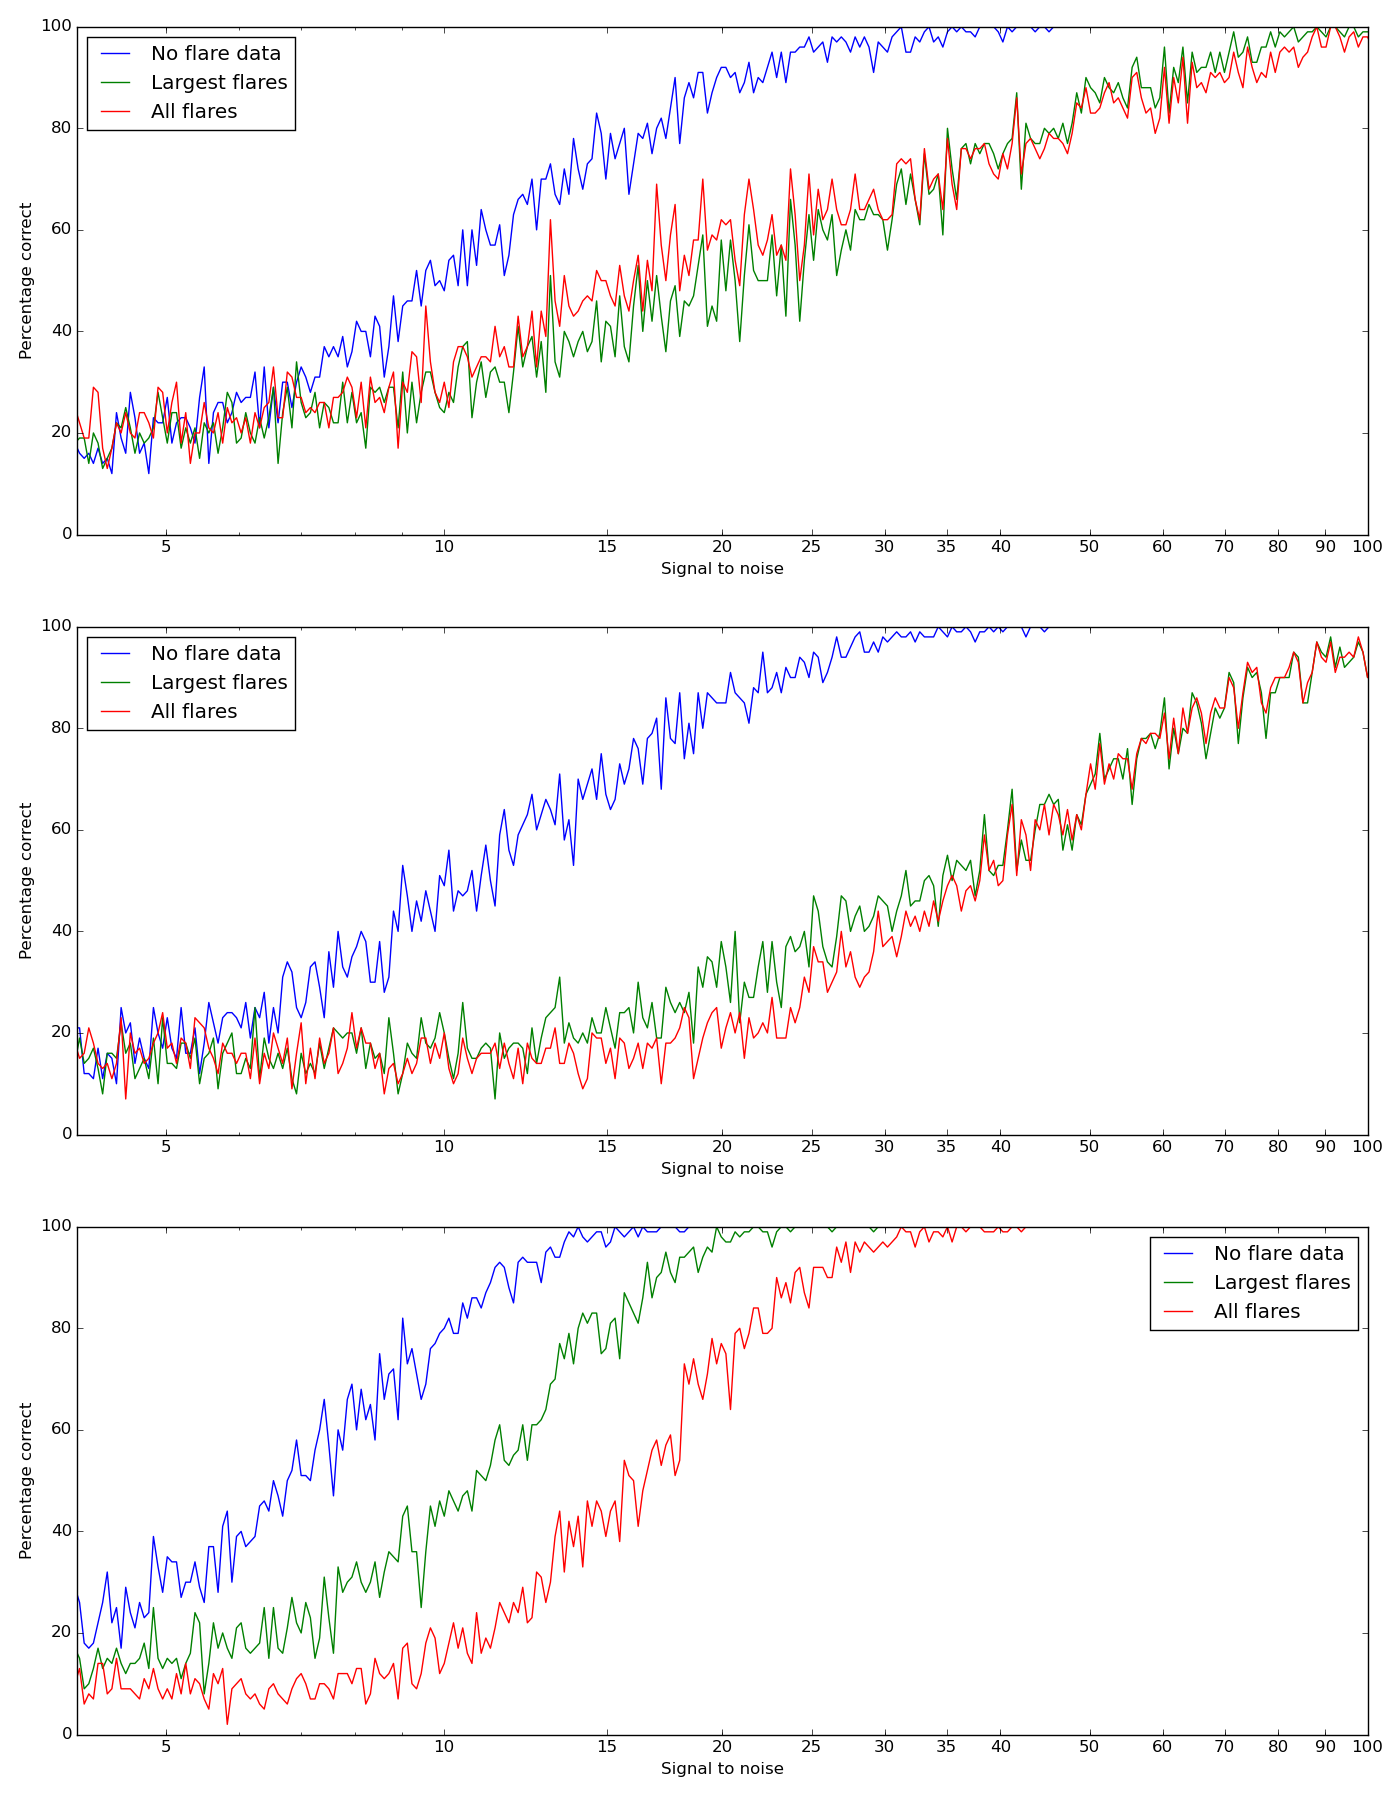
\includegraphics[scale=0.25]{Figures/Np80.png} \\
\end{center}
\caption{This figure shows the percentage of the correctly recovered period of 80 days as the strongest peak with
  various levels of SNR and adding various levels of simulated flare data, the blue plot for no flare data. the green
  plot with the four largest flare data (up to the January 2014) and the red plot the flare data clipped in Section
  \ref{section:harpsper} as having equivalent width greater than 1 standard deviation from the median in the original
  data to January 2014.  The topmost panel shows the results for an inclination of 30{\degree}, the middle panel that
  for 60{\degree} and the bottom panel for 90{\degree}.}
\protect\label{fig:noiseresults}
\end{figure}

It was of interest to note the impact of the rotation period on these results, in Fig. \ref{fig:noiseresults60} is shown
effectively the same data as Fig. \ref{fig:noiseresults}, but with a period of 60 days instead of 80 days. It was
noticeable how this performed significantly better than the 80-day period, closer to the 82.6-day period calculated for
\prox. Further reductions in the period improved the recovery still further, in a relationship apparently better than
linear (although many more simulations, in terms of numbers of runs and length of periods, would be required to
establish this with accuracy), lending weight to the contention that the spectroscopic line measurements are likely to
prove of more value with stars with a faster rotation period than \prox.

\begin{figure}[!htbp]
\begin{center}
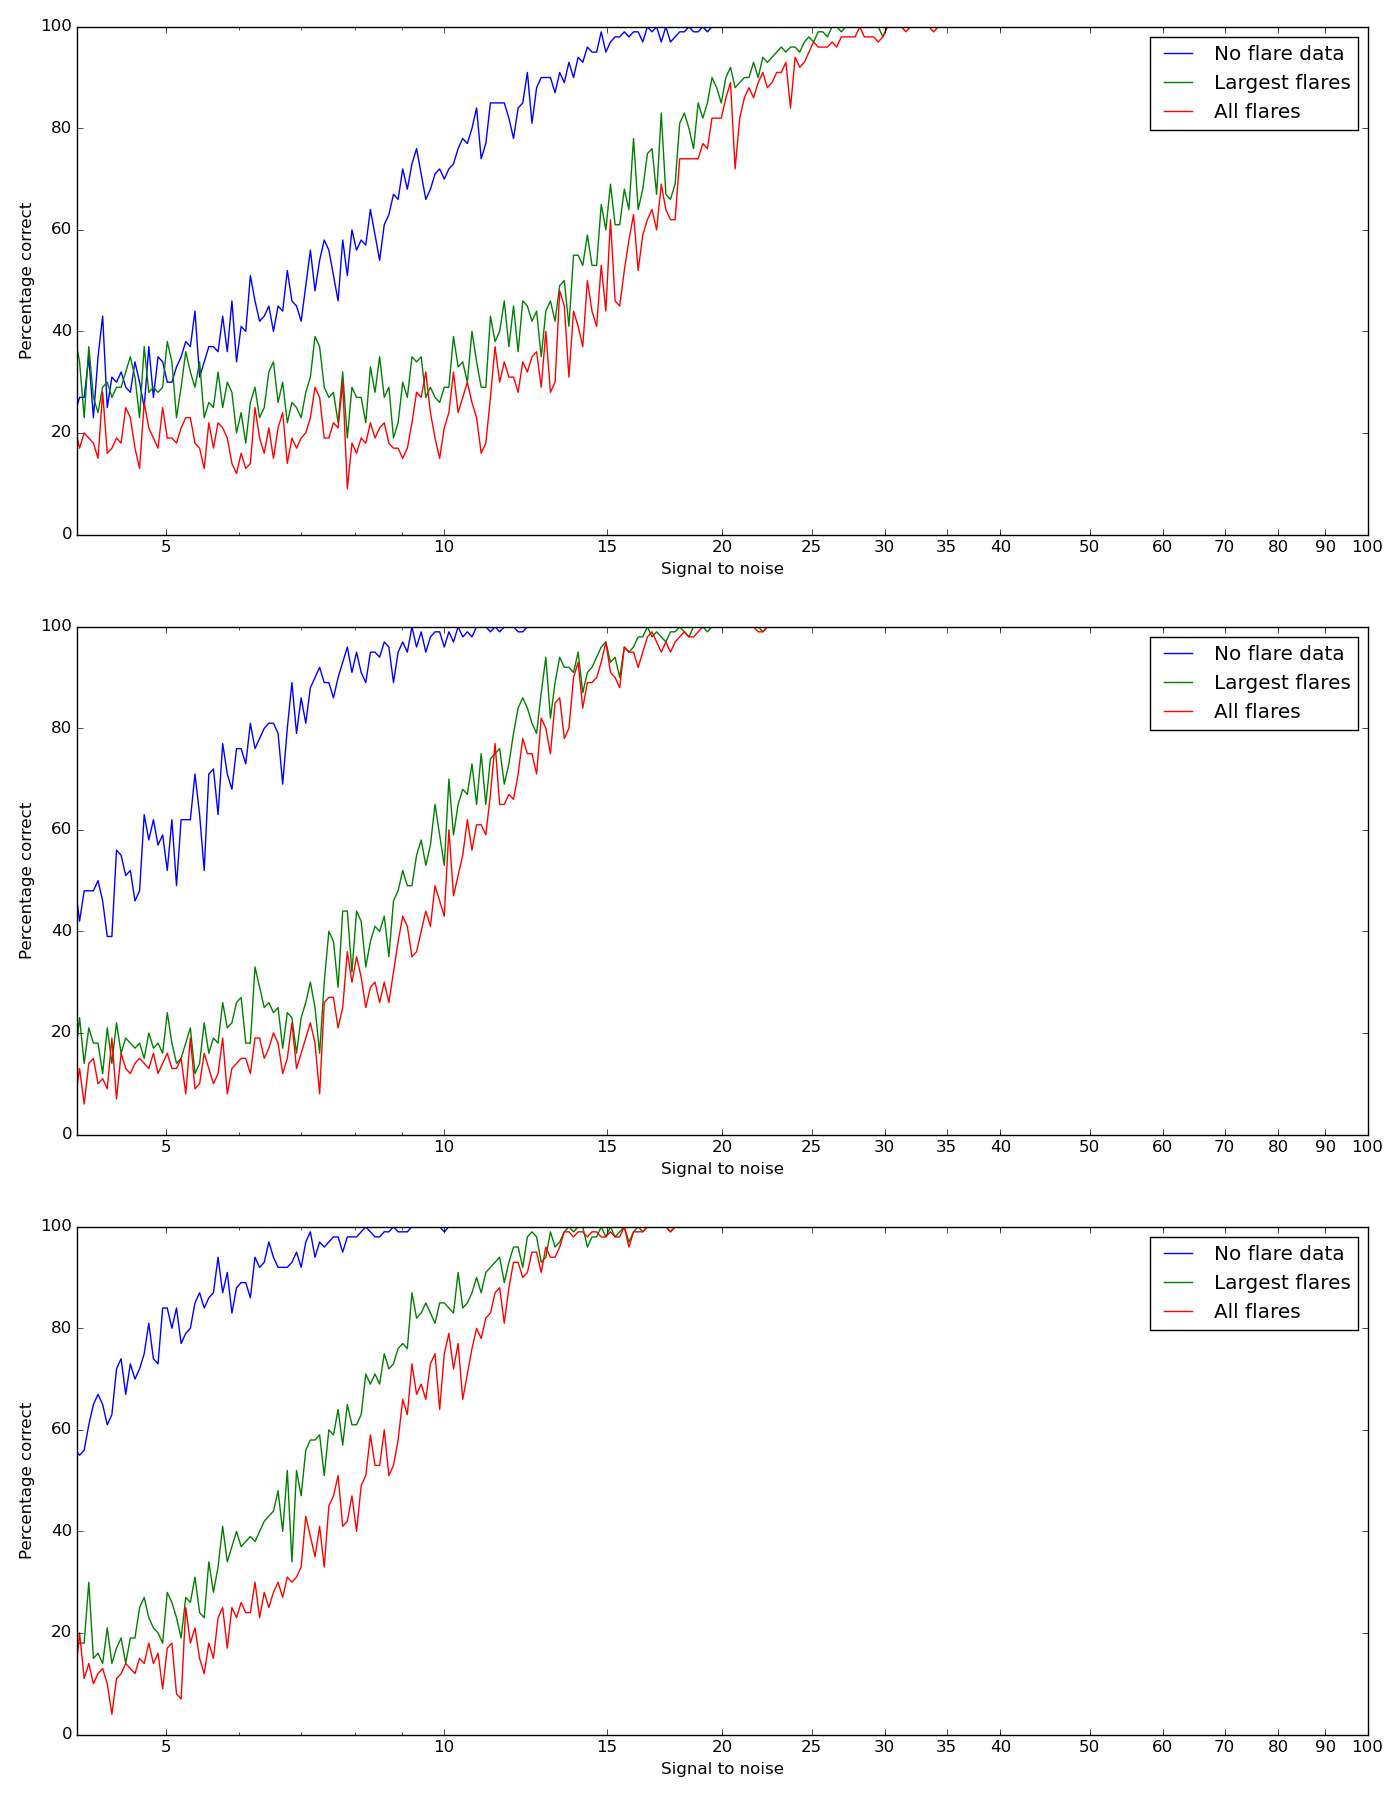
\includegraphics[scale=0.25]{Figures/Np60.png} \\
\end{center}
\caption{This figure is effectively the same as Fig. \ref{fig:noiseresults}, but from a starting period of 60 rather
  than 80 days, showing the significant improvement in the recovery rates with the shorter period.}
\protect\label{fig:noiseresults60}
\end{figure}

Some of the false positives from these simulations were noted and in quite a few cases it was noticed that periods close
to 116.6 days reported in \citet[Table 3]{suarezmascareno15} appeared as one of the prominent peaks in the modelling
results. An example is shown in Fig. \ref{fig:rec116}. This period is clearly an artefact of the observation times,
which were copied from the Original Set of {\harps} data for use in the model. \examrevision{This is further confirmed
  by the period \examrevisiona{of 116.5} being observed in the window function for those observation times as previously
  shown in Fig. \ref{fig:harpswfos}.}

\begin{figure}[!htbp]
\begin{center}
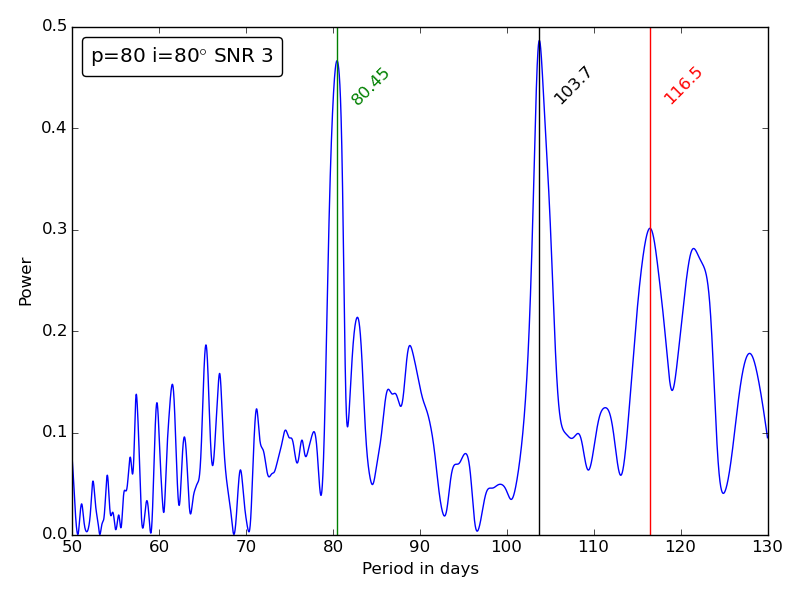
\includegraphics[scale=0.4]{Figures/badeg.png} \\
\end{center}
\caption{Example of a periodogram from the modelling simulations after adding noise which returns a peak close to 116.6
days.This was from a case where no flare data was added, to a model based on a period of 80 days, an inclination given
of 80{\degree} and a SNR of 3. Here 116.5 days appears as the third-strongest peak (highlighted in red). This example
gives the strongest peak as 103.7 days, marked in black and the correct period as 80.45 days, marked in green.}
\protect\label{fig:rec116}
\end{figure}
